\chapter{Концепции симуляции}\label{chap:lab02}

\section{Цель занятия}

В данной работе продолжается изучение принципов работы симулятора Simics. Центральная тема занятия --- определение способов представления сущностей реальных устройств и систем в программных моделях.

\subsection{Базовая единица симуляции} 

Аналогично тому, что физические системы строятся из узлов, программные платформы состоят из моделей отдельных узлов. При этом, как и в реальности, они образуют иерархическую структуру.

\subsection{Диагностические сообщения}

Одно из назначений симуляторов --- помогать в разработке аппаратуры и программ для неё. При этом разработчикам необходимо понимать, что происходит в системе в определённые моменты времени. Для этого всем моделям позволено создавать диагностические сообщения, которые могут выводится на консоль управления Simics, а также в файл. Поскольку излишне частые и подробные сообщения могут засорить журнал, Simics предоставляет несколько механизмов для их фильтрации.

\section{Ход работы}

Запустите симулятор с моделируемой системой внутри:

\begin{lstlisting}
$ ./simics -e '$cpu_class=core-i7-single' targets/x86-x58-ich10/viper-busybox.simics
\end{lstlisting}

\subsection{Иерархия устройств}

Корневой элемент созданной модели компьютера имеет имя, хранящееся в переменной \texttt{\$system}. В нашем случае это \texttt{viper} --- модель шасси, на котором <<крепятся>> все остальные устройства. Этот факт выражается в том, что иерархические имена подкомпонент образованы присоединением к имени надкомпоненты своего имени через символ точки. Так, материнская плата данной системы имеет имя \texttt{viper.mb}, процессор на ней --- \texttt{viper.mb.cpu0}, а первое ядро в этом процессоре --- \texttt{viper.mb.cpu0.core[0][0]}.

Для просмотра списка всех устройств используйте команду \texttt{list-objects -recursive}. Альтернативно можно использовать окно \textbf{Object Browser} (рис.~\ref{fig:object-browser}).

\begin{figure}[htb]
    \centering
    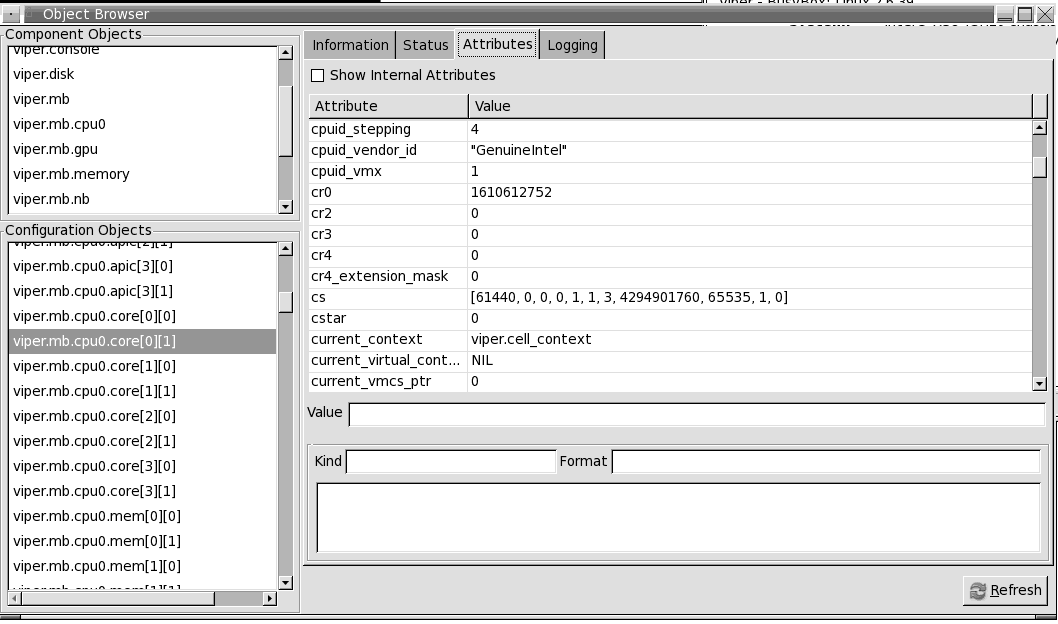
\includegraphics[width=0.8\textwidth]{/win-object-browser}
    \caption{Окно для просмотра объектов и их атбрибутов}
    \label{fig:object-browser}
\end{figure}


\subsection{Команды}

Каждый класс моделей может предоставлять несколько команд, которые позволяют инспектировать или изменять состояние объектов данного класса. Такие команды приписываются к иерархическому имени модели.

Самые часто реализуемые внутри классов команды --- это \texttt{status} и \texttt{info}.

Так же все устройства модели памяти имеют команды \texttt{get} и \texttt{set}, которые позволяют читать и записывать данные в симулируемую память. Например:

\begin{lstlisting}
simics> viper.mb.cpu0.mem[0][0].get address = 0xffff0000

simics> viper.mb.cpu0.mem[0][0].set address = 0xffff0000 value = 0xaabbccdd
\end{lstlisting}


\subsubsection{Глобальные команды}

Кроме команд, специфичных для устройств, существуют так называемые глобальные команды, эффект которых состоит или в доступе к состоянию всей симуляции в целом, или же к текущему <<устройству>> некоторого класса, что позволяет сэкономить время на наборе иерархических имён. Например, команда \texttt{ptime} выводит значения симулируемого времени для текущего процессора, тогда как \texttt{ptime -all} позволяет увидеть аналогичную информацию о всех процессорах в системе.

\begin{lstlisting}
simics> ptime
processor                 steps   cycles   time[s]
viper.mb.cpu0.core[0][0]      0        0         0
\end{lstlisting}


\subsection{Атрибуты}

Атрибуты являются аналогом полей классов в парадигме ООП. В симуляции основная их задача состоит в хранении архитектурного состояния моделей. Обратиться к ним можно по их имени, указываемому после имени объекта, с помощью оператора <<\texttt{->}>>:

Например, для просмотра регистров центрального процессора можно использовать соответствующие атрибуты:
\begin{lstlisting}
simics> viper.mb.cpu0.core[0][0]->rax
0
simics> viper.mb.cpu0.core[0][0]->rip
65520
simics> viper.mb.cpu0.core[0][0]->rdx
67233
simics> viper.mb.cpu0.core[0][0]->xmm
[[0, 0], [0, 0], [0, 0], [0, 0], [0, 0], [0, 0], [0, 0], [0, 0], [0, 0], [0, 0], [0, 0], [0, 0], [0, 0], [0, 0], [0, 0], [0, 0]]
\end{lstlisting}

Для изменения значения, хранимого в атрибуте, используется оператор присваивания <<\texttt{=}>>:
\begin{lstlisting}
simics> viper.mb.cpu0.core[0][0]->rax = 123
\end{lstlisting}

\subsubsection{Типы атрибутов}

По аналогии с переменными в языках программирования атрибуты имеют типы. При присвоении атрибуту нового значения предварительно производится проверка, что тип выражения с правой стороны соответсвует его заявленному типу.

Типы атрибутов специфицируются с помощью строки, символы которой определяют допустимые варианты входных значений.

\begin{enumerate*}
\item Скалярные. Имеют типы \texttt{i}, \texttt{s}, \texttt{b}.
\item Объекты. Их тип --- \texttt{o}.
\item Списки. Они могут быть как однородными \texttt{[iiii]}, так и содержать элементы разных типов \texttt{[oios]}. Кроме того, их длина может быть переменной: \texttt{[i*]}.
\item Пустой тип \texttt{n}.
\item Допустимо иметь атрибут, тип которого выбирается из нескольких ранее описанных: \texttt{i|s|o}.

\end{enumerate*}

Кроме того, некоторые атрибуты при регистрации могут быть помечены как псевдоатрибуты или атрибуты только для чтения. Почти всегда они не соответствуют архитектурному состоянию, а используются для удобства представления информации об устройстве или же могут быть выведены из содержимого других атрибутов.

\subsection{Интерфейсы}

Каждый интерфейс имеет уникальное имя и фиксированный набор методов, объединённых общей целью. Модель, желающая предоставлять некоторый интерфейс для других устройств, обязана реализовать один или несколько его методов и затем объявить его доступным. Стороннее устройство, имеющее ссылку на объект, может получить по нему заявленные интерфейсы и вызывать включённые в него методы. Таким образом, в Simics интерфейсы предоставляют объектно-ориентированную парадигму для взаимодействия отдельных моделей. 

Например, один из атрибутов процессора, настраиваемый на этапе инициализации модели, --- это \texttt{physical_memory}, его тип \texttt{o}, т.е. <<объект>>. Допустим, что \texttt{cpu->physical_memory = mem}. По указателю на объект \texttt{mem} процессор может извлечь из него реализацию интерфейса \texttt{memory-space}, который содержит методы \texttt{read}, \texttt{write}, \texttt{access} и др. для работы с пространствами памяти.

В данной работе мы не будем уделять много внимания  деталям работы с интерфейсами. Отметим лишь, что все команды любого устройства внутри себя написаны с использованием только его атрибутов и интерфейсов, т.к. не существует другого способа взаимодействий с ним. Однако устройства должны взаимодействовать друг с другом только через интерфейсы, но не атрибуты.

\subsection{Модули устройств}

С точки зрения организации хранения в Simics любая модель предоставляется ровно одним \textit{модулем} --- разделяемой библиотекой, загружаемой на этапе инициализации или позже. При этом модуль может предоставлять более одного класса моделей.

Для просмотра текущих загруженных модулей используйте команду:

\begin{lstlisting}
simics> list-modules -l
\end{lstlisting}

Для загрузки некоторого модуля вручную используется команда \texttt{load-module}.

Кроме того, некоторые найденные модули по той или иной причине могут быть отвергнуты при загрузке. Увидеть их список можно с помощью команды \texttt{list-failed-modules}.

% \subsection{Псевдоустройства}
% 
% Для унификации работы с различными сущностями в активной сессии Simics присутствуют также псевдоустройства, такие как \texttt{sim}, \texttt{prefs}, \texttt{sysmon} и др.

\subsection{Последовательность создания модели системы}

При создании симуляции она и все участвующие в ней объекты проходят две фазы, чётко отделённые друг от друга во времени, тогда как внутри каждой из них порядок инициализации компонент неопределён.

\begin{enumerate*}

\item \textit{Объявление} устройств и соединение их с помощью инициализации их атрибутов. На этом этапе ещё не произодится проверок на соответствие типов, наличие всех обязательных атрибутов. Устройства представлены так называемыми предобъектами (\abbr preobj).

\item \textit{Инстанциирование} устройств с помощью команды \texttt{instantiate-components}. На этом этапе производятся все проверки на корректность атрибутов, наличие необходимых интерфейсов. Если не найдено ошибок, то предобъекты преобразуются в полноценные объекты Simics, которые могут участввать в симуляции.

\end{enumerate*}

Отметим, что при необходимости добавить новые объекты в процессе симуляции описанные фазы могут быть повторены.

\section{Задания}

 В этой работе мы будем создавать небольшую симуляцию, состоящую из простой модели процессора класса \texttt{sample-risc} и модели оперативной памяти. Для этого необходимо будет создать и настроить индивидуальные объекты. Исходный скрипт находится в файле \texttt{script.py} (см. приложение~\ref{chap:app-broken-script}). Однако он содержит несколько ошибок, которые не позволяют это сделать сразу. Задание состоит в том, чтобы разобрать сообщения симулятора, внести модификации в исходный скрипт и запустить его.

Следующие замечания должны помочь в решении поставленной задачи.

\begin{itemize*}
    \item Данный скрипт написан на языке Python и поэтому требует специального флага при указании его имени в командной строке.
    \item Для выяснения списка опций используйте команду \texttt{simics -h}.
    \item Переменные в Simics объявляются с помощь оператора <<\texttt{=}>>. Имена переменных начинаются со знака доллар, например \texttt{\$system}.
    \item Перед выполнением второй фазы инициализации объектов все обязательные атрибуты предобъектов должны быть настроены.
    \item Обращайте внимание на вывод сообщения об ошибках --- часто они содержат имя файла и номер строки.
    \item Комментарии начинаются со знака <<диез>> \texttt{\#}.
\end{itemize*}

\iftoggle{webpaper}{
    \printbibliography[title={Список литературы к занятию}]
}{}